\documentclass{gnulike}
\usepackage{natbib}
\usepackage{graphics}
\usepackage{chngcntr}
\usepackage{sectsty}
\usepackage{rotating}
\usepackage{emptypage}
\usepackage[titletoc]{appendix}

\let\leqslant=\leq

%\newcommand{\psm}{small-scale physical modeling method}
%\newcommand{\bialt}{\textit{BiAlt} }
%\newcommand{\cmnt}[1]{}

\DeclareMathSizes{10}{10}{10}{10}

\definecolor{light-gray}{gray}{0.95}
\definecolor{bashgray}{RGB}{209,214,217}
\newcommand{\addbash}[1]{
	\begin{center}
	\colorbox{bashgray}{\begin{minipage}{0.9\textwidth}
  	\ttfamily \$ #1
\end{minipage}}
	\end{center}
}


\usepackage[dvipsnames]{xcolor}
\usepackage{minibox}

\usepackage{graphicx}
\usepackage{color}

\definecolor{vibrisblue1}{RGB}{90,151,190}
\definecolor{vibrisblue2}{RGB}{25,96,177}

\newcommand{\indice}[1]{\scriptsize{#1}}
\newcommand{\subtitle}{FDPSV}

\titleformat{\chapter}[hang] 
{\normalfont\huge\bfseries}{\thechapter}{0.5em}{} 
\titlespacing*{\chapter}{0pt}{-20pt}{20pt}

\usepackage{makeidx}
\makeindex

\mdseries

\begin{document}

\begin{titlepage}
  \newpage
  \null
  \vskip 10.0em
  \let\center\flushleft
  {\noindent \huge{\bf SWAM2D} \par}
  \vskip -0.5em
  {\noindent \rule{\textwidth}{0.3em} \par}

  {\hfill Documentation for SWAM2D version 0.1 \par}
  
  {\hfill 18 January 2017 \par}
  
  \vfill
  
  {\noindent \Large{Damien Pageot}}
  \vskip -0.5em
  {\noindent \rule{\textwidth}{0.2em} \par}
  \vskip 1.0cm
\end{titlepage}

% ----------------------------------------------------------------------
% MANUAL LICENSE
% ----------------------------------------------------------------------
\null\vfill
\pagenumbering{gobble}
\noindent Copyright \copyright\ 2016-2017 Damien Pageot.\\

\noindent Permission is granted to copy, distribute and/or modify this document under the terms of the GNU Free Documentation License, Version 1.3 or any later version published by the Free Software Foundation; with no Invariant Sections, no Front-Cover Texts, and no Back-Cover Texts. A copy of the license is included in the section entitled "GNU Free Documentation License".
\clearpage\newpage

% ----------------------------------------------------------------------
% TABLE OF CONTENTS
% ----------------------------------------------------------------------
\pagenumbering{roman}
\tableofcontents
\thispagestyle{empty}
\clearpage\newpage

\pagenumbering{arabic}
% ----------------------------------------------------------------------
% INTRODUCTION
% ----------------------------------------------------------------------
\chapter{Introduction}
\index{Introduction}

% ----------------------------------------------------------------------
% THEORETICAL BACKGROUND
% ----------------------------------------------------------------------
\chapter{Theoretical background}

\noindent test $\Sigma$, $\Xi$, $\mathsf{T}$

\begin{eqnarray}
  \frac{\partial v_{x}}{\partial t} = \rho^{{\scriptscriptstyle-1}} \left( \frac{\partial \tau_{xx}}{\partial x} + \frac{\partial \tau_{xz}}{\partial z} \right) \\
  \frac{\partial v_{z}}{\partial t} = \rho^{{\scriptscriptstyle -1}} \left( \frac{\partial \tau_{xz}}{\partial x} + \frac{\partial \tau_{zz}}{\partial z} \right) \\
  \frac{\partial \tau_{xx}}{\partial t} = (\lambda+2\mu)\frac{\partial v_{x}}{\partial x} + \lambda \frac{\partial v_{z}}{\partial z} \\
  \frac{\partial \tau_{zz}}{\partial t} = (\lambda+2\mu)\frac{\partial v_{z}}{\partial z} + \lambda \frac{\partial v_{x}}{\partial x} \\
  \frac{\partial \tau_{xz}}{\partial t} = \mu \left( \frac{\partial v_{x}}{\partial z} + \frac{\partial v_{z}}{\partial x } \right)
\end{eqnarray}

\section{Equation of motion}
\index{equation of motion}

\section{Staggered grid}
\index{staggered grid}

\cite{virieux1986psv,levander1988fourth}

\begin{figure}[!ht]
  \centering
  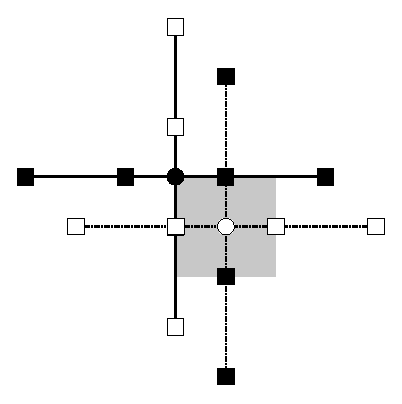
\includegraphics[width=0.9\textwidth]{fig/staggered.eps}
  \caption{Staggered finite-difference grid and spatial stencils for (a) the velocity update and (b) the stress update. After \cite{levander1988fourth} with velocity-stress position switch proposed by \cite{bohlen2006accuracy}.}
  \label{fig:staggered-grid}
\end{figure}

\noindent Second order forward ($D^{+}$) and backward ($D^{-}$) operators:
\index{forward operator}
\index{backward operator}
\begin{eqnarray}
  D^{+}=f(i+1)-f(i) \nonumber \\
  D^{-}=f(i)-f(i-1)
\end{eqnarray}

\noindent Fourth-order forward ($D^{+}$) and backward ($D^{-}$) operators:
\begin{eqnarray}
  D^{+}=c_{1}[f(i+1)-f(i)]+c_{2}[f(i+2)-f(i-1)] \nonumber \\
  D^{-}=c_{1}[f(i)-f(i-1)]+c_{2}[f(i+1)-f(i-2)]
\end{eqnarray}


\index{Lam\'e parameters}
\index{parameter harmonization}
\begin{eqnarray}
  \bar{\mu}(i+\frac{1}{2}, j+\frac{1}{2})=\frac{1}{4}(\mu(i,j)+\mu(i+1,j)+\mu(i,j+1)+\mu(i+1,j+1) \\
  \rho_{x}(i,j+\frac{1}{2}) = \frac{1}{2}(\rho (i,j+1)+\rho(i,j)) \\
  \rho_{z}(i+\frac{1}{2},j) = \frac{1}{2}(\rho (i+1,j)+\rho(i,j))
\end{eqnarray}

\section{Initial and boundary conditions}
\index{absorbing boundary condition}
\index{free surface condition}

\subsection{Perfectly Matched Layer (PML)}
\index{perfectly matched layer}

\cite{berenger1994perfectly}

\begin{eqnarray}
\label{pml-damp}
d = d_{0} \left( \frac{q}{L_{PML}} \right) ^{n} \\
d_{0} = 3c_{p} \frac{log(1/R)}{2L_{PML}}
\end{eqnarray}

\subsection{Free surface}
\index{free surface}

% ----------------------------------------------------------------------
% GETTING STARTED
% ----------------------------------------------------------------------
\chapter{Getting started}

\section{Requirements}

\noindent For FDPSV program:
\begin{itemize}
	\item GNU make $>=$ 4.1
	\item GNU gfortran $>=$ 4.7
\end{itemize}

\noindent Optional for examples:
\begin{itemize}
	\item python $>=$ 2.7
	\item python-numpy $>=$ 1.8.2
\end{itemize}

\noindent Optional:
\begin{itemize}
	\item Seismic Un*x $>=$ 43R1
\end{itemize}

\subsection{Compilation}
\addbash{make}

% ----------------------------------------------------------------------
% INPUT PARAMETERS AND FILES
% ----------------------------------------------------------------------
\section{Input parameters and files}
\index{input parameters}
\index{input files}

% ----------------------------------------------------------------------
% NUMERICAL EXAMPLES
% ----------------------------------------------------------------------
\chapter{Numerical examples}

\begin{appendices}
% ----------------------------------------------------------------------
% APPENDICES
% ----------------------------------------------------------------------
%\chapter{Finite-difference equations}
\index{finite-difference equations}
\chapter{Finite-difference equations}

\begin{equation}
  E(i,j)=\lambda(i,j)+2\mu (i,j)
\end{equation}

\begin{eqnarray}
  D_{t}^{+}v_{x}^{t}({\scriptstyle i,j+1/2,l-1/2}) = \rho_{x}^{-1}({\scriptstyle i,j}) [D_{x}^{+}\tau_{xx}({\scriptstyle i,j,l})+D_{z}^{-}\tau_{xz}({\scriptstyle i+1/2,j,l})] \\
  D_{t}^{+}v_{z}^{t}({\scriptstyle i+1/2,j,l-1/2}) = \rho_{z}^{-1}({\scriptstyle i,j}) [D_{x}^{-}\tau_{xz}({\scriptstyle i+1/2,j+1/2,l})+D_{z}^{+}\tau_{zz}({\scriptstyle i,j,l})] \\
  D_{t}^{+}\tau_{xx}({\scriptstyle i,j,l}) = E({\scriptstyle i,j}) D_{x}^{-}v_{x}({\scriptstyle i,j+1/2,l+1/2})+\mu({\scriptstyle i,j}) D_{z}^{-}v_{z}({\scriptstyle i+1/2,j,l+1/2}) \\
  D_{t}^{+}\tau_{zz}({\scriptstyle i,j,l}) = \mu({\scriptstyle i,j}) D_{x}^{-}v_{x}({\scriptstyle i,j+1/2,l+1/2})+ E({\scriptstyle i,j}) D_{z}^{-}v_{z}({\scriptstyle i+1/2,j,l+1/2})\\
  D_{t}^{+}\tau_{xz}({\scriptstyle i+1/2,j+1/2,l}) = \bar{\mu}({\scriptstyle i+1/2,j+1/2})[D_{z}^{+}v_{x}({\scriptstyle i,j+1/2,l+1/2}) +D_{x}^{+}v_{z}({\scriptstyle i+1/2,j,l+1/2})]  
\end{eqnarray}


%\chapter{GNU Free Documentation License}
\index{GNU FDL}  
\input{fdl-1.3}

\end{appendices}
  
% ----------------------------------------------------------------------
% References
% ----------------------------------------------------------------------

\bibliography{references}

\clearpage
\newpage
\thispagestyle{empty}
\printindex

\end{document}
